\documentclass{beamer}
%\documentclass[aspectratio=169]{beamer}
%\usetheme{Madrid} % My favorite!
%\usetheme{Boadilla} % Pretty neat, soft color.
%\usetheme{default}
%\usetheme{Warsaw}
%\usetheme{Bergen} % This template has nagivation on the left
\usetheme{Frankfurt} % Similar to the default 
%with an extra region at the top.
\usecolortheme{seahorse} % Simple and clean template
%\usetheme{Darmstadt} % not so good
% Uncomment the following line if you want %
% page numbers and using Warsaw theme%
% \setbeamertemplate{footline}[page number]
%\setbeamercovered{transparent}
\setbeamercovered{invisible}
% To remove the navigation symbols from 
% the bottom of slides%
\setbeamertemplate{navigation symbols}{} 
%
\usepackage{graphicx}
\usepackage[backend=biber,]{biblatex}

\addbibresource{AAAI-Spring-Symposium.bib}
\bibliographystyle{amsalpha}
\usepackage{tikz}
\usepackage{calc}
\def\checkmark{\tikz\fill[scale=0.4](0,.35) -- (.25,0) -- (1,.7) -- (.25,.15) -- cycle;} 
\def\scalecheck{\resizebox{\widthof{\checkmark}*\ratio{\widthof{x}}{\widthof{\normalsize x}}}{!}{\checkmark}}
%that's defined it - now for a test

\DeclareGraphicsExtensions{.pdf,.png,.jpg}
%\usepackage{bm}         % For typesetting bold math (not \mathbold)
%\logo{\includegraphics[height=0.6cm]{yourlogo.eps}}
%
\title[Multi-Vector Trust]{A Multi-Vector Trust Framework for Autonomous Systems}
\author{Andrew Bolster, Alan Marshall}
\institute[UoL]
{
University of Liverpool \\
\medskip
{\emph{andrew.bolster@liv.ac.uk, alan.marshall@liv.ac.uk}}\\
\vspace{0.3in}

\includegraphics[width=0.5\textwidth]{img/livuni}%
}
\date{\today}
% \today will show current date. 
% Alternatively, you can specify a date.
%
\begin{document}
%

%\AtBeginSection[
%{
%\begin{frame}<beamer>{Table of Contents}
%  \tableofcontents[currentsection,currentsubsection, 
%  hideothersubsections, 
%  sectionstyle=show/shaded,
%  ]
%\end{frame}
%}]
\begin{frame}
  \titlepage
\end{frame}

\frame{\tableofcontents}

\section{Trust Management Frameworks in Ad-Hoc Systems}
\subsection{What do we mean by trust?}
\frame{
\frametitle{Trust in Ad-Hoc Systems and the context of this document}
\begin{itemize}
  \item Particularly interested in the application of Trust in Decentralised (P2P) Autonomous Systems of Systems, Autonomous Underwater Vehicles (AUVs) for example
  \item <2->Trust:\emph{The expectation of an actor performing a certain task or range of tasks within a certain confidence or probability}
  \item<3->Full System Views of Trust
    \begin{itemize}
      \item<3->{Design Trust - that a system of systems will perfom as spec'd / designed in operation}
      \item<4>{Operational Trust - the systems within a larger system will perfom as designed in field \checkmark}
    \end{itemize}
\end{itemize}
}
\subsection{What are TMFs?}
\frame{
\frametitle{Trust Management Frameworks}
\begin{itemize}
  \item Provide information regarding the estimated future states and operations of nodes within networks
  \item <2->``[\ldots]collecting the information necessary to establish a trust relationship and dynamically monitoring and adjusting the existing trust relationship'' - \footfullcite{Li2007}
  \item <3->Enables nodes to form collaborative \emph{opinions} on their cohort nodes based on
    \begin{itemize}
      \item Direct Observation of Communications Behaviour (eg Successfully Forwarded Packets)
      \item Common-Neighbour Recommendation
      \item Indirect Reputation
    \end{itemize}
\end{itemize}
}
\frame{
\frametitle{Transitivity in Trust Networks}
\begin{center}
  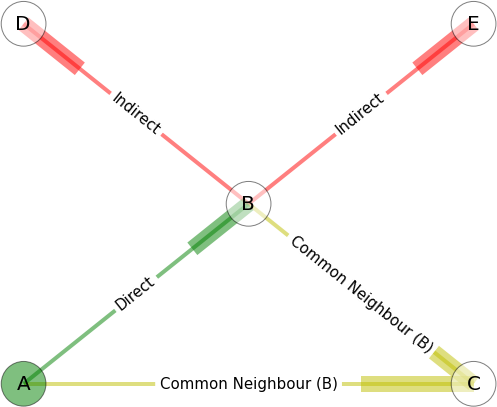
\includegraphics[height=0.6\paperheight]{img/node_relationships}
\end{center}
}

\subsection{Reasons for using Communication TMFs}
\frame{
\frametitle{TMFs in Ad Hoc Autonomous Systems}
\begin{itemize}
  \item Multiple transitive relationships can be maintained over time, providing trust resilience with dyanmic network topology
  \item<2->Enable trust establishment from partial-strangers via indirect trust and direct observation
  \item<3->Enables nodes to inform internal processes for global efficiency given observed network behaviour / 'wellness', similar to those found in human social networks eg
    \begin{itemize}
      \item Update routing table based on 'safest' node chains (Phone Tree)
      \item Maneuver away from misbehaving nodes (Shunning)
      \item Inform as to 'trustworthiness' of forwarded information (Healthy sense of Skepticism)
      \item Historic Distrust/Trust decaying over time (Forgiveness/Relationship Decay)
    \end{itemize}
\end{itemize}
}
\frame{
\frametitle{Reason for using TMFs in MANETs}
\begin{itemize}
  \item Provide Risk Mitigation against many classical MANET attacks
    \begin{itemize}
      \item Black/Grayhole
      \item Routing Loop
      \item Selective misbehaviour / selfishness
    \end{itemize}
  \item Generally; to constrain potential malicious behaviour that can operate without detection
\end{itemize}
}

\subsection{Pre-existing Research}
\frame{
\frametitle{Trust in Autonomous Systems}
\begin{itemize}
  \item Public Key Infrastructure - Requires Centralised Control and pre-shared keys
  \item Resurrecting Duckling - Uses in-action keying with a trusted source
  \item Evidence Based Trust - Uses shared keys 
  \item Reputation Based Trust - Uses Packet forwarding success rate for prediction of future actions
    \begin{itemize}  
      \item CONFIDANT - Trust-based router implementation using packet forwarding rate
      \item OTMF - Trust including transitive information from otehr nodes
      \item <2-> MTMF - Relationships and Multiple Metrics combined with Gray Interval assessment
    \end{itemize}
  \item \ldots and there are plenty more along the same lines
\end{itemize}
}


\section{Vectorised Trust, Multi-vector Trust and Gray Theory}
\subsection{Vector Trust}
\frame{
\frametitle{Vectorised Trust}
\begin{itemize}
  \item Application of several individual metrics for the construction of a single trust measurement
  \item For example:
    \begin{itemize}
      \item $X=\{packet\ loss, signal\ strength, data rate, delay, throughput\}$
    \end{itemize}
  \item This multi-parameter trust prevents 'smart' attackers; leveraging a known trust metric to subvert a TMF without detection
  \item Normally expressed as a vector, but can be condensed into an abstracted or weighted form for comparison \cite{Guo2012}
\end{itemize}
}

\subsection{Gray Theory}
\frame{
\frametitle{Gray Theory and it's Application in MTMF }
\begin{itemize}
  \item
    \begin{math}
      \big[\theta_{k,j},\phi_{k,j}\big]^t=\Big[\frac{\min_k{|a_{kj}^t-g_j^t|+\rho \max_k{|a_{kj}^t-g_j^t|}}}{\max_k{|a_{kj}^t-g_j^t|}t},\frac{\min_k{|a_{kj}^t-b_j^t|+\rho \max_k{|a_{kj}^t-b_j^t|}}}{\max_k{|a_{kj}^t-b_j^t|}t}\Big]
    \end{math}\cite{Zuo:1995:DMG:202081.202086}
  \item <1->Basically, scale the individual values against the global maximum and minimum of the sample set to obtain an interval
  \item <2->
    \begin{math}
      \big[\theta_{k},\phi_{k}\big]^t= \sum\limits_{j=1}^m h_j \big[\theta_{k,j}^t,\phi_{k,j}^t\big]
    \end{math}
  \item <3->
    \begin{math}
      T_k^t = \frac{1}{1+\frac{(\phi_k^t)^2}{(\theta_k^t)^2}}\\
      T_{k,tot}^t = T_k^t + T_{k,net}^t + (\alpha \times T_k^{t-1} + (1-\alpha) \times T_{k,tot}^{t-1})
    \end{math}

\end{itemize}
}
\frame{
\frametitle{Malicious Behaviour Discrimination}
\begin{center}
  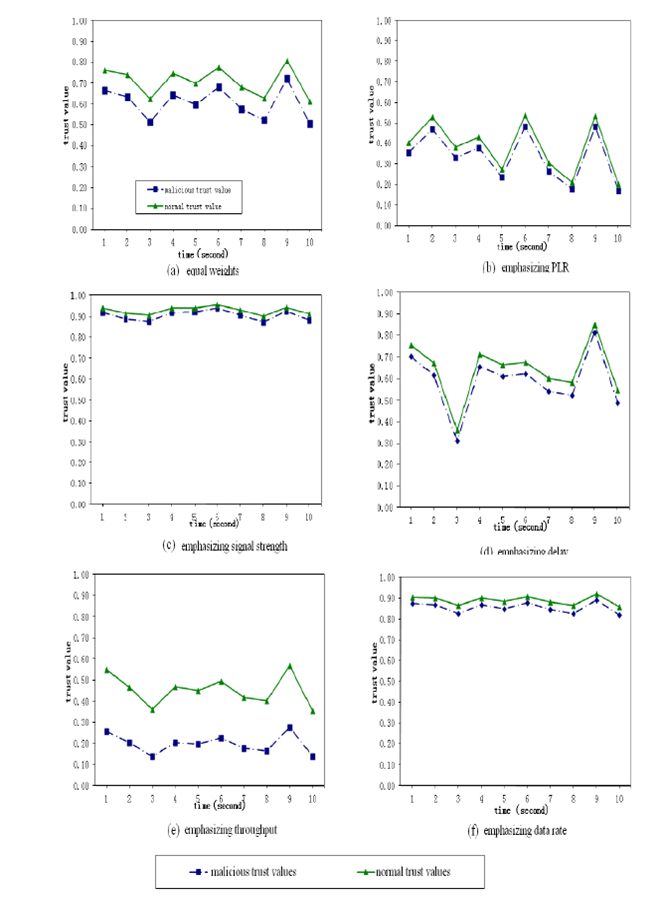
\includegraphics[height=0.8\paperheight]{img/bellas_vector_detector}
\end{center}
}



\subsection{Multi-Vector Trust}
\frame{
\frametitle{Agent Based Behaviour Simulator}
\begin{center}
  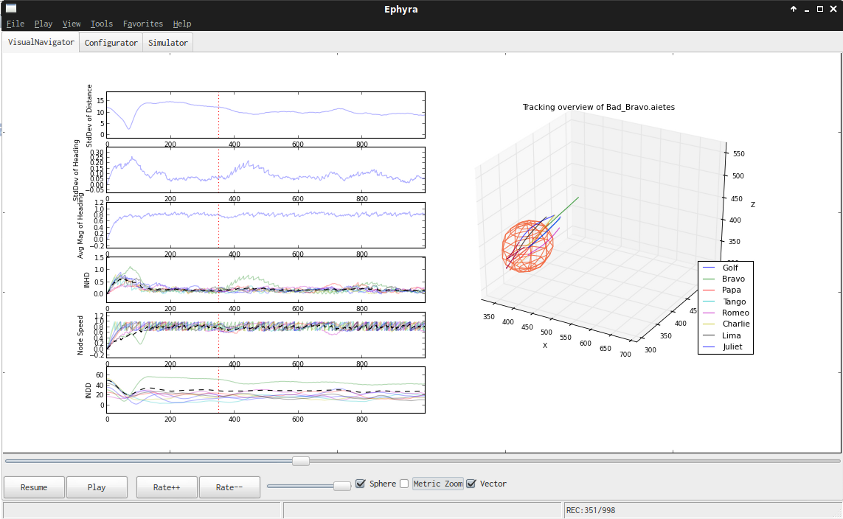
\includegraphics[width=0.9\paperwidth]{img/ephyra_vis}
\end{center}
}

\frame{
\frametitle{Multi-Vector Trust and the Threat Surface}
Potential attacks exist across a multi-domain threat surface
\begin{center}
  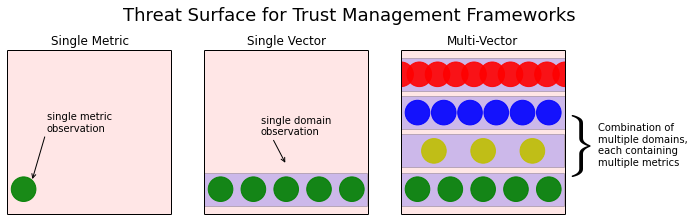
\includegraphics[width=0.9\paperwidth]{img/threat_surface_sum}
\end{center}
}
\frame{
\frametitle{Trust in Mobile Autonomous Underwater Vehicles}
\begin{itemize}
  \item Flocking with Intent: MCM, Port Protection, Survey, Protection Detail, etc.
  \item<2-> Metric Selection in collaboration CMRE/DSTL
    \begin{itemize}
      \item Inter Node Heading Deviation
      \item Inter Node Distance Deviation
      \item Node Speed
    \end{itemize}
  \item <3-> Behaviour selection for testing
    \begin{itemize}
      \item Shadow
      \item Slowcoach
      \item Spy
      \item Sloth
    \end{itemize}

\end{itemize}
}
\frame{
\frametitle{Raw Behavioural Metric Assessment in AUVs}
\begin{center}
  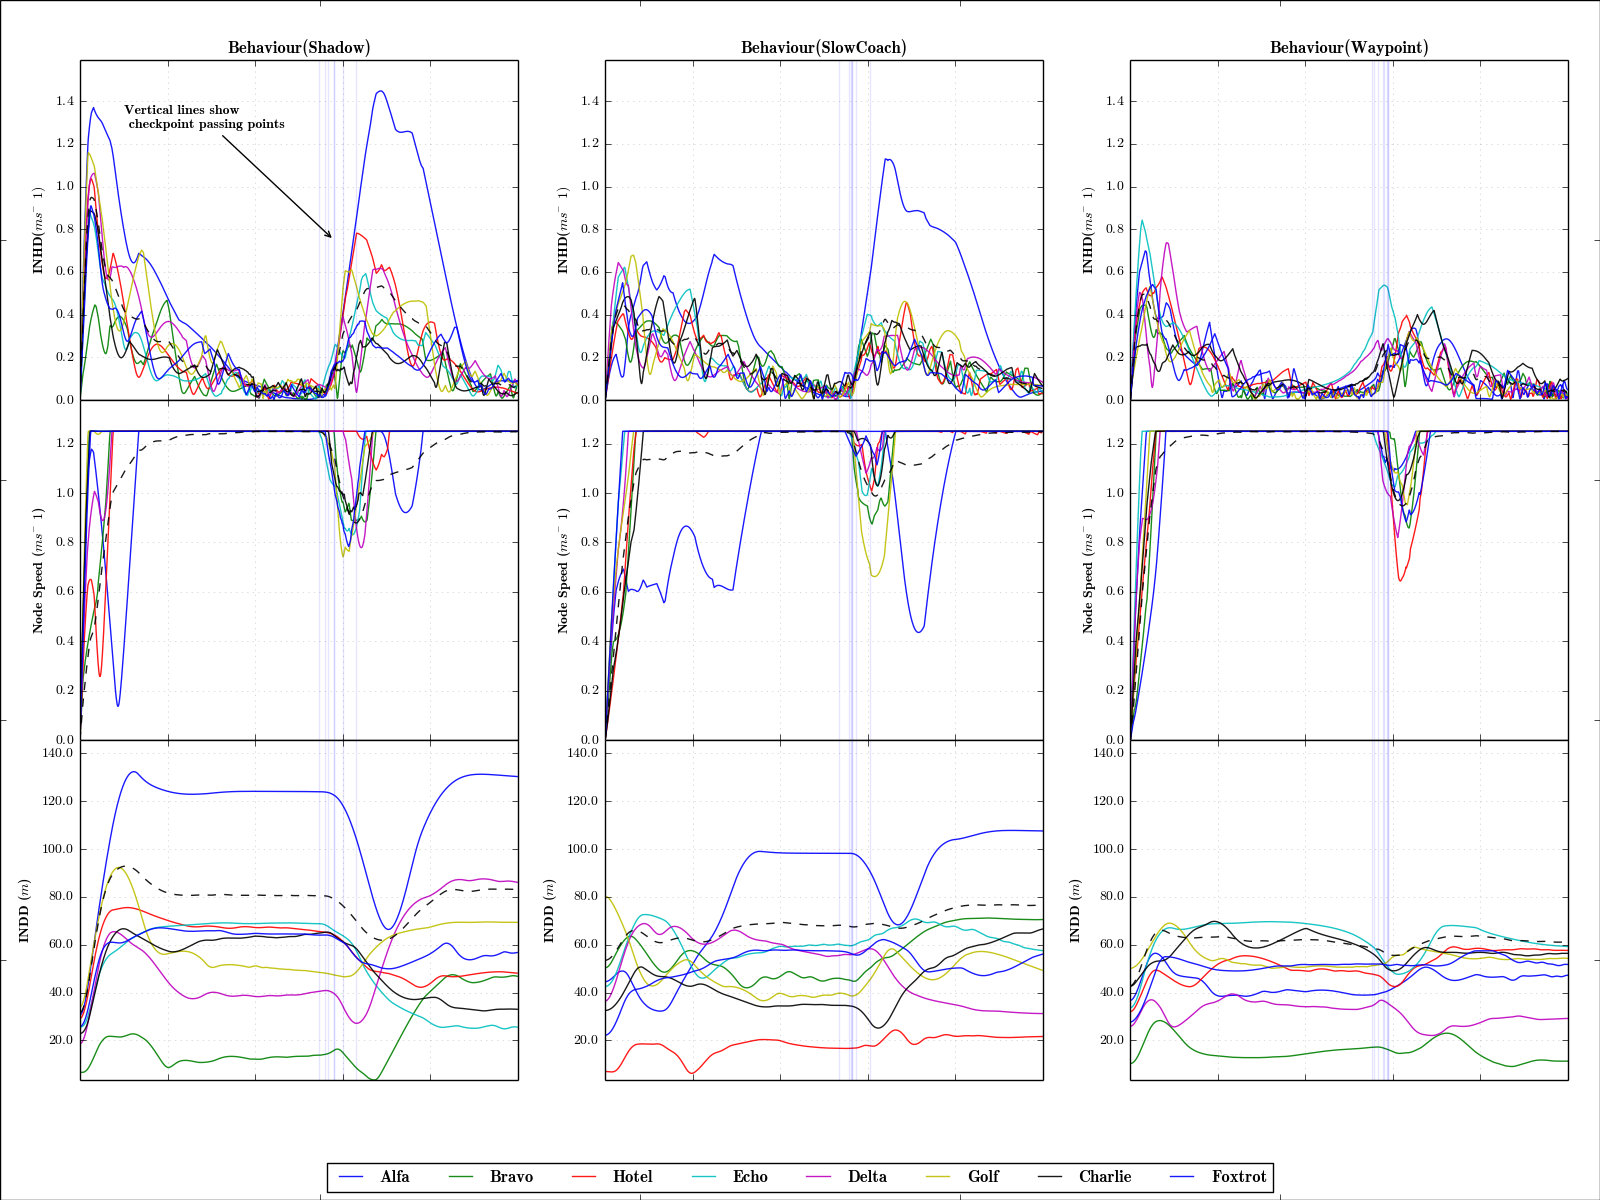
\includegraphics[height=0.8\paperheight]{img/BehaviourMetricComparison}
\end{center}
}
\frame{
\frametitle{Behavioural Trust Assessment in AUVs}
\begin{center}
  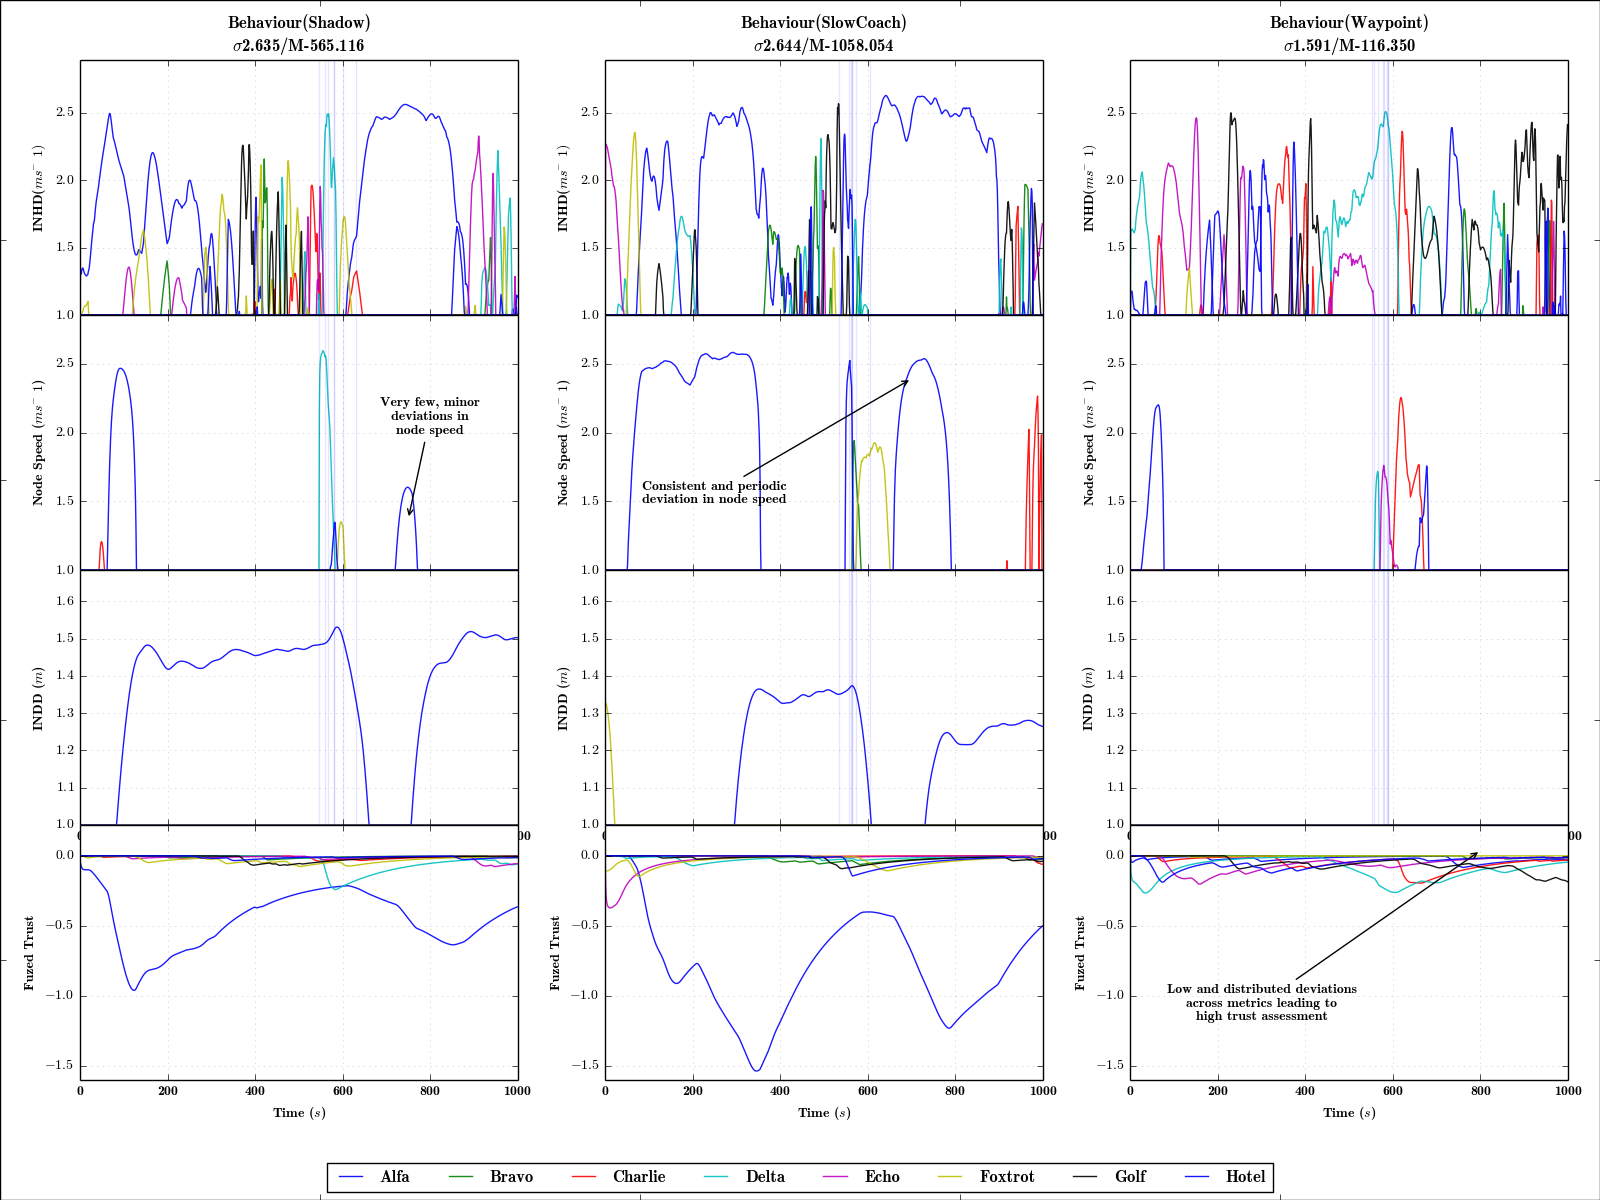
\includegraphics[height=0.8\paperheight]{img/BehaviourFusion}
\end{center}
}
\subsection{Challenges for Implementing Multi-vector Trust}
\frame{
\frametitle{Challenges in Multi-vector Trust}
\begin{itemize}
  \item How to define optimality in trust assessment when dealing with multiple vectors and transitive trust?
  \item Is there a quantifiable benefit to cross-domain comparison beyond single vector Trust?
  \item Is there an optimal generic cross-domain comparator?
\end{itemize}
}


%
\begin{frame}
  \frametitle{References}
  \printbibliography% [nottype=video]}
\end{frame}

\begin{frame}
  \centerline{The End}
\end{frame}
% End of slides
\end{document} 


